\documentclass[border=10pt]{standalone}
\usepackage[american, siunitx]{circuitikz}
\usetikzlibrary{calc, positioning}

\begin{document}
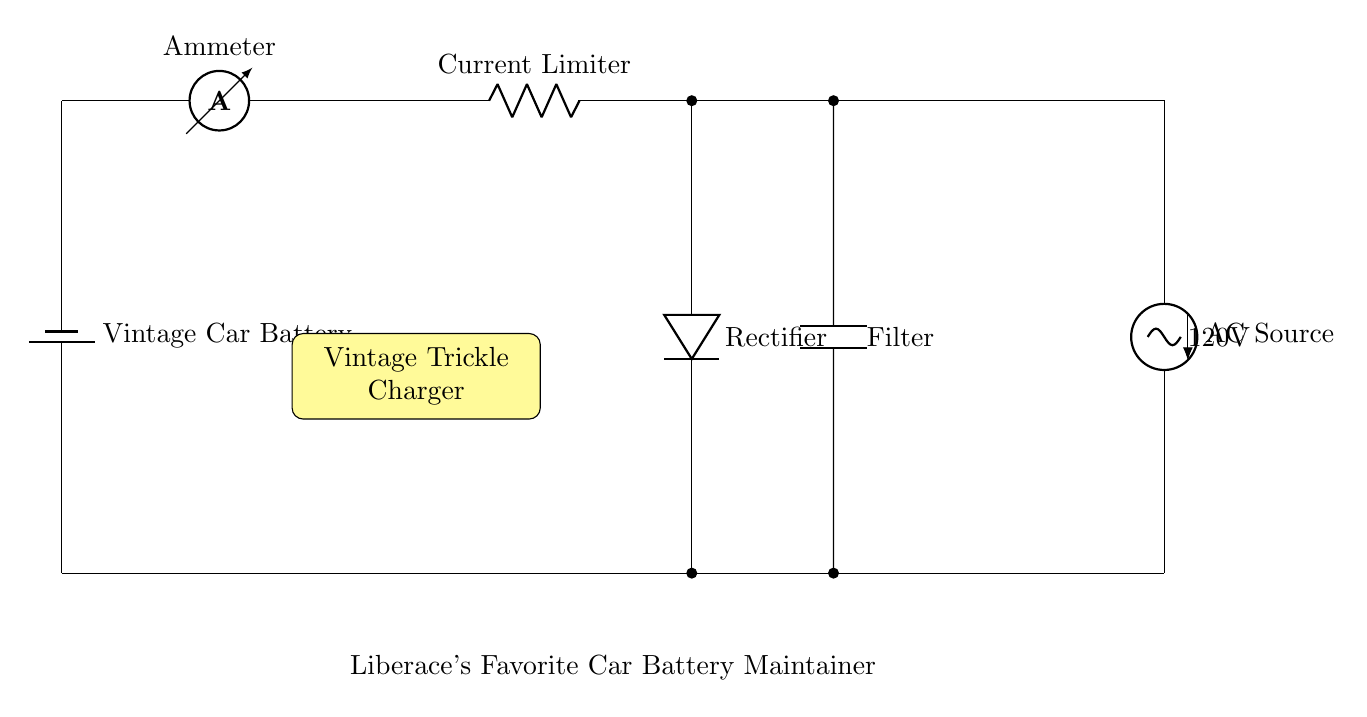
\begin{tikzpicture}[
    circuitikz/label/align = straight,
    font=\rmfamily
]
    % Define coordinates for the main loop corners
    \def\W{14}
    \def\H{6}
    \coordinate (bl) at (0,0);
    \coordinate (tl) at (0,\H);
    \coordinate (br) at (\W,0);
    \coordinate (tr) at (\W,\H);

    % Draw bottom and left parts of the loop
    \draw (bl) to[battery1, l_={Vintage Car Battery}] (tl);
    \draw (bl) -- (br);

    % Draw top path components
    \draw (tl) to[ammeter, l=Ammeter] (4,\H) to[R, l=Current Limiter] (8,\H) coordinate (shunt_node);
    \fill (shunt_node) circle (2pt);

    % Draw right part of the loop (AC source)
    \draw (shunt_node) -- (tr) to[sV, l={AC Source}] (br);
    
    % Add 120V label and arrow next to AC source
    \node at (\W, \H/2) [right=0.5em] {120V};
    \draw[-{Latex}] (\W+0.3, \H/2+0.3) -- ++(0,-0.6);

    % Draw the shunt rectifier/filter branch
    \coordinate (shunt_bot) at (shunt_node |- bl);
    \fill (shunt_bot) circle (2pt);
    
    % Diode (Rectifier)
    \coordinate (diode_mid) at ($(shunt_node)!0.5!(shunt_bot)$);
    \draw (shunt_node) to[D] (shunt_bot);
    \node[right=0.3cm of diode_mid] {Rectifier};

    % Capacitor (Filter) in parallel with diode
    \coordinate (cap_top) at ($(shunt_node)+(1.8,0)$);
    \coordinate (cap_bot) at (cap_top |- bl);
    \coordinate (cap_mid) at ($(cap_top)!0.5!(cap_bot)$);
    
    \draw (shunt_node) -- (cap_top);
    \draw (shunt_bot) -- (cap_bot);
    \draw (cap_top) to[C] (cap_bot);
    \node[right=0.3cm of cap_mid] {Filter};
    
    \fill (cap_top) circle (2pt);
    \fill (cap_bot) circle (2pt);

    % Add central yellow box
    \node[draw, rounded corners, fill=yellow!40, text width=2.8cm, align=center, inner sep=5pt] at (4.5, \H/2 - 0.5) {Vintage Trickle \\ Charger};

    % Add bottom caption
    \node at (\W/2, -1.2) {Liberace's Favorite Car Battery Maintainer};

\end{tikzpicture}
\end{document}